\documentclass{article}

% Language setting
% Replace `english' with e.g. `spanish' to change the document language
\usepackage[english]{babel}

% Set page size and margins
% Replace `letterpaper' with `a4paper' for UK/EU standard size
\usepackage[a4paper,top=2cm,bottom=2cm,left=3cm,right=3cm,marginparwidth=1.75cm]{geometry}

% Useful packages
\usepackage{amsmath}
\usepackage{graphicx}
\usepackage{dirtytalk}
\usepackage[table]{xcolor}% http://ctan.org/pkg/xcolor
\usepackage[colorlinks=true, allcolors=blue]{hyperref}

\title{Examples for Machine Learning}
% \author{Luis Brocai}

\begin{document}
\maketitle

\say{If I had more time, I would have written a shorter letter.}

\newpage

\section{Introduction}

\subsection{Power set}
The power set is the set of all subset.
For example, let $A = \{1, 2, 3\}$
\begin{equation*}
2^A = \{ \{\}, \{1\}, \{2\}, \{3\}, \{1, 2\}, \{1,3\}, \{2,3\}, \{1,2,3\}\}    
\end{equation*}
In this example, there are $8 = 2^3 = 2^{|A|}$ elements in the power set.
In general $|2^A| = 2^{|A|}$, hence the notation.

\subsection{m-elementary subsets}
The set of all m-elementary subsets is denoted by $\binom{A}{m}$.
For example, let $A = \{1, 2, 3\}$.
\begin{equation*}
    \binom{A}{2} = \{ \{1, 2\}, \{1,3\}, \{2,3\} \}.
\end{equation*}
In this example, there are $3 = \binom{3}{2} = \binom{|A|}{2}$ elements in the set (\href{https://en.wikipedia.org/wiki/Binomial_coefficient}{binomial coefficient}).
In general $ |\binom{A}{2}| = \binom{|A|}{2}$, hence the notation.

\subsection{set of all maps from A to B}
The set of all maps from A to B is denoted by $B^A$.
For example let $A = \{x, y\}$ and $B = \{1, 2, 3\}$.
\begin{equation*}
    \begin{split}
        B^A = \{&(x \mapsto 1, y \mapsto 1), \\
        &(x \mapsto 1, y \mapsto 2), \\
        &(x \mapsto 1, y \mapsto 3), \\
        &(x \mapsto 2, y \mapsto 1), \\
        &(x \mapsto 2, y \mapsto 2), \\
        &(x \mapsto 2, y \mapsto 3), \\
        &(x \mapsto 3, y \mapsto 1), \\
        &(x \mapsto 3, y \mapsto 2), \\
        &(x \mapsto 3, y \mapsto 3)\}
    \end{split}
\end{equation*}

In this example, there are $9 = 3^2 = |B|^{|A|}$ elements in the set.
In general $ |B^A| = |B|^{|A|}$, hence the notation.

\newpage


\section{Supervised learning}
The general idea will be presented, once we had an example.

\section{Learning of DNFs}

\subsection{Disjunctive Normal Forms}

DNFs always look a bit like this:
\begin{equation*}
    (x_1 \land x_2 \land x_4) \lor (x_1 \land \lnot x_2) \lor (x_2 \land \lnot x_3)
\end{equation*}
It's some and-clauses (conjunctions) joined in one big or-clause (disjunction), hence the name. If we are using 0 and 1 instead of booleans, we can represent an and by multiplying the variables ($x_1 \land x_2 = x_1 * x_2$) and negation as 1 - x ($\lnot x_1 = (1 - x_1)$). I will stick with the boolean notation as I find it more intuitive, even though in the lecture the product notation is chosen to be more consistent with the labelling using 0 and 1. Just know that {0, 1} and {false, true} will be used somewhat interchangeably here.

\subsection{Example}

Let's start with an example. Our function / program will take some input about attributes of a city and should return, whether the city is a good choice to live in.
The attributes for each city will be
\begin{enumerate}
\item Are the housing prices high? (yes/no)
\item Does the city have a high population? (yes/no)
\item Is the public transport system good? (yes/no)
\end{enumerate}
And the decision will be
\begin{itemize}
\item Is the city livable? (yes/no)
\end{itemize}
The inputs and outputs are binary decisions (yes/no) which can be represented by booleans (true/false) or binary labels (1/0).
Our function should take in the attributes of a city and use a DNF (disjunctive normal form) to output a decision for the city.
Our DNF for deciding, whether a city is livable could look something like this:
\begin{equation*}
    (\lnot x_{costly} \land x_{transport})
\end{equation*}
Notice, this is a DNF with just one and-clause, which is why there is no $\lor$ required.
It also doesn't make use of all attributes (it skips population).
This DNF would label all cities with low costs and good transport as a livable city. All other cities would not be considered livable. This sounds reasonable, but we are not just interested in finding something that sounds reasonable. We are interested in finding something that fits some labeled data we are given.

\subsubsection{Labeled Data}

The data we are given could look something like this.
\begin{itemize}
    \item Dresden
    \begin{itemize}
        \item $x_{costly} = 0$ (low housing prices)
        \item $x_{populated} = 1$ (high population (for German standards))
        \item $x_{transport} = 1$ (good public transport)
        \item $y = 1$ (It's a good city to live in)
    \end{itemize}
    
    \item Heidelberg
    \begin{itemize}
        \item $x_{costly} = 1$
        \item $x_{populated} = 0$
        \item $x_{transport} = 1$
        \item $y = 1$
    \end{itemize}
    
    \item Stuttgart
    \begin{itemize}
        \item $x_{costly} = 1$
        \item $x_{populated} = 1$
        \item $x_{transport} = 1$
        \item $y = 0$ (I just needed something with a zero, Stuttgart isn't that bad)
    \end{itemize}
\end{itemize}

It could also be written in a table like this:

\begin{center}
    \begin{tabular}{c || c c c | c}
        & costly & populated & transport & livable \\
        \hline
        \hline
        Dresden & 0 & 1 & 1 & 1 \\
        Heidelberg & 1 & 0 & 1 & 1 \\
        Stuttgart & 1 & 1 & 1 & 0 \\
    \end{tabular}
\end{center}


The formal notation will be presented in the following paragraphs.

\subsubsection{S: Set of Samples}

S is our set of samples:

\begin{equation*}
S = \{Dresden, Heidelberg, Stuttgart\}
\end{equation*}

\subsubsection{X: Set of all possible attribute assignments}

Our attributes are denoted by V.

\begin{equation*}
    V = \{costly, populated, transport\}
\end{equation*}

In the lecture our attributes are often defined more generally with just $V = \{1, 2, 3\}$.
Every attribute can take on the value 0 or 1. Thus, our set of all possible attribute assignments, denoted by X, will look like this:

\begin{equation*}
    \begin{split}
        X = \{&0, 1\}^V \\
         = \{&(costly \mapsto 0, populated \mapsto 0, transport \mapsto 0), \\
        &(costly \mapsto 0, populated \mapsto 0, transport \mapsto 1), \\
        &(costly \mapsto 0, populated \mapsto 1, transport \mapsto 0), \\
        &(costly \mapsto 0, populated \mapsto 1, transport \mapsto 1), \\
        &(costly \mapsto 1, populated \mapsto 0, transport \mapsto 0), \\
        &(costly \mapsto 1, populated \mapsto 0, transport \mapsto 1), \\
        &(costly \mapsto 1, populated \mapsto 1, transport \mapsto 0), \\
        &(costly \mapsto 1, populated \mapsto 1, transport \mapsto 1)\}
    \end{split}
\end{equation*}

\subsubsection{x: Matching attribute assignments to cities}

Assigning cities one of the attribute assignments will be done with a map x from the samples to some elements of X.

$(x: S \rightarrow X)$:
\begin{equation*}
    \begin{split}
        x = \{&Dresden \mapsto (costly \mapsto 0, populated \mapsto 1, transport \mapsto 1), \\
        &Heidelberg \mapsto (costly \mapsto 1, populated \mapsto 0, transport \mapsto 1), \\
        &Stuttgart \mapsto (costly \mapsto 1, populated \mapsto 1, transport \mapsto 1)\}
    \end{split}
\end{equation*}

\subsubsection{y: Labels for cities}

The labels for the cities (whether they are livable or not) are defined in a map y from S to 0 or 1.

$(y: S \rightarrow \{0, 1\})$:

\begin{equation*}
    y = (Dresden \mapsto 1, Heidelberg \mapsto 1, Stuttgart \mapsto 0)
\end{equation*}

\subsection{Deciding}
We now try to find the best DNF that takes in the attributes of a city and returns the correct label for this city.
The DNF defined earlier, which was just a guess, looked like this:
\begin{equation*}
    (\lnot x_{costly} \land x_{transport})
\end{equation*}

It would map Dresden as follows:
\begin{equation*}
    Dresden: (\lnot x_{costly} \land x_{transport}) = \lnot false \land true = true       
\end{equation*}

Or with $\{0, 1\}$:

\begin{equation*}
    Dresden: (1 - x_{costly}) * x_{transport} = (1 - 0) * 1 = 1       
\end{equation*}

It would correctly assess that Dresden is a livable city. However, it would incorrectly label Heidelberg as a non-livable city. So our goal now is to find among all possible DNFs ($\Theta$) one that correctly maps all cities to their respective label.

\subsubsection{Formal Notation of a DNF}

A DNF like this
\begin{equation*}
    (\lnot x_{costly} \land \lnot x_{populated} \land x_{transport}) \lor (x_{costly} \land x_{populated})
\end{equation*}
will be represented as a set. Each element in the set corresponds to one and-clause. Each of these and-clauses is represented by a tuple $(V_0, V_1)$, where $V_0$ defines the variables that occur in the negated form in the and-clause and $V_1$ defines the variables that occur in the non-negated form in the and-clause. The DNF above would become
\begin{equation*}
    \{(\{x_{costly}, x_{populated}\}, \{x_{transport}\}), (\{\}, \{x_{costly}, x_{population}\}\}
\end{equation*}

The set of all possible and-clauses can then be defined as $\Gamma = \{(V_0, V_1) \in 2^V \times 2^V | V_0 \cap V_1 = \emptyset \}$. The restriction $V_0 \cap V_1 = \emptyset$ states that a variable cannot occur in it's negated and non-negated form at the same time. The set of all DNFs $\Theta$ then is all disjunctions that can be built by using elements of the set of all conjunctions $\Gamma$. So $\Theta = 2^\Gamma$.

\subsubsection{Complexity of DNFs}
Two way of judging the complexity of DNFs are depth and length. The regularizer $R_l$ for length counts the total number of variables that occur in the DNF. The regularizer $R_d$ for depth counts the number of variables in the longest and-clause withing the DNF. The following DNF has a length of 5 and a depth of 3.

\begin{equation*}
    (\lnot x_{costly} \land \lnot x_{populated} \land x_{transport}) \lor (x_{costly} \land x_{populated})
\end{equation*}


\subsubsection{Learning Problem}
The supervised learning problem asks us to find a DNF that gets the labelling correct, while keeping complexity low. How relevant correctness is compared to complexity is determined by a parameter $\lambda$. We want to find a $\theta$ to minimize

\begin{equation*}
    \lambda * R(\theta) + (1-\lambda) * averageLoss(\theta)
\end{equation*}

Let's look at our example. The first DNF we came up with
\begin{equation*}
    (\lnot x_{costly} \land x_{transport})
\end{equation*}
mapped Dresden and Stuttgart correctly, but failed for Heidelberg. The loss for a sample is 0, if the labelling was correct and 1 if the labelling was incorrect. The total loss is therefore:
\begin{equation*}
\sum_{s \in S} L(f_\theta(x_s), y_s) = 0 + 0 + 1 = 1
\end{equation*}
The average loss then is $\frac{1}{3}$. The length is 2 and depth is also 2. 


By looking at the labeled data that is mapped to 1 we can also define a DNF that maps everything correctly:
\begin{equation*}
    (\lnot x_{costly} \land x_{populated} \land x_{transport}) \lor
    (x_{costly} \land \lnot x_{populated} \land x_{transport})
\end{equation*}
Since this DNF gets every label right, the total and average loss are 0. However, the length is 6 and depth is 3. So depending on how we weigh correctness vs complexity (and whether we look at depth or length), both of the two DNFs could be more suitable for some given requirements than the other.

\subsection{Generalizing learning problems}
Our goal was to find a good DNF, that can correctly decide for some input data, whether a city is livable or not.
To define what a good DNF is we looked at two aspects:

\begin{enumerate}
    \item Correctness: We are given some labeled data. The DNF ($\theta$) should be chosen/learned in such a way, that the function gets this training data right. To measure this, we use the Loss function L.
    \item Complexity: The function should not be too complicated and have small length or depth. To measure this, we use the regularizer R.
\end{enumerate}

In general, we are interested in finding a good $\theta$, which has little loss and small complexity. $\theta$ could describe the structure of a DNF, but also the structure of a Binary Decision Tree or parameters in a neural network.

\subsection{Bounded Depth DNF Problem}

A different learning problem is the bounded depth DNF problem. It asks us to get every label right, while restricting the depth (longest and-clause) to some limit m.
Both of the examples above fail to be a solution of a \textsc{depth-2-dnf}. One doesn't get everything correct, the other one has a depth over 2.

A suitable solution would be:

\begin{equation*}
    (\lnot x_{costly} \land x_{populated}) \lor
    (x_{costly} \land \lnot x_{populated})
\end{equation*}

\subsubsection{Hardness of finding solutions to \textsc{depth-m-DNF}}
Finding a solution to the \textsc{depth-m-dnf} problem for large inputs is hard. For a growing number of attributes and labeled data, the time to find a solution grows at least exponentially in our best known algorithms. In fact, we can show that finding a solution would also allow us to find solutions to problems, for which there is believed to be no algorithm better than exponential time growth. One such problems is \textsc{set-cover}.

\paragraph{\textsc{set-cover}}

We are given some sets $\Sigma = \{\{a, b\}, \{b\}, \{c, d\}\}$ and another set $S' = \{a, b, c, d\}$ which we are supposed to cover using only m (for example m=2) sets from $\Sigma$. As suitable cover for m=2 would be $\sigma_1 = \{a, b\}$ and $\sigma_3 = \{c, d\}$. This problem is known to be hard to solve as the inputs grow larger.

\paragraph{Purpose of a reduction}

\begin{figure}[h]
    \centering
    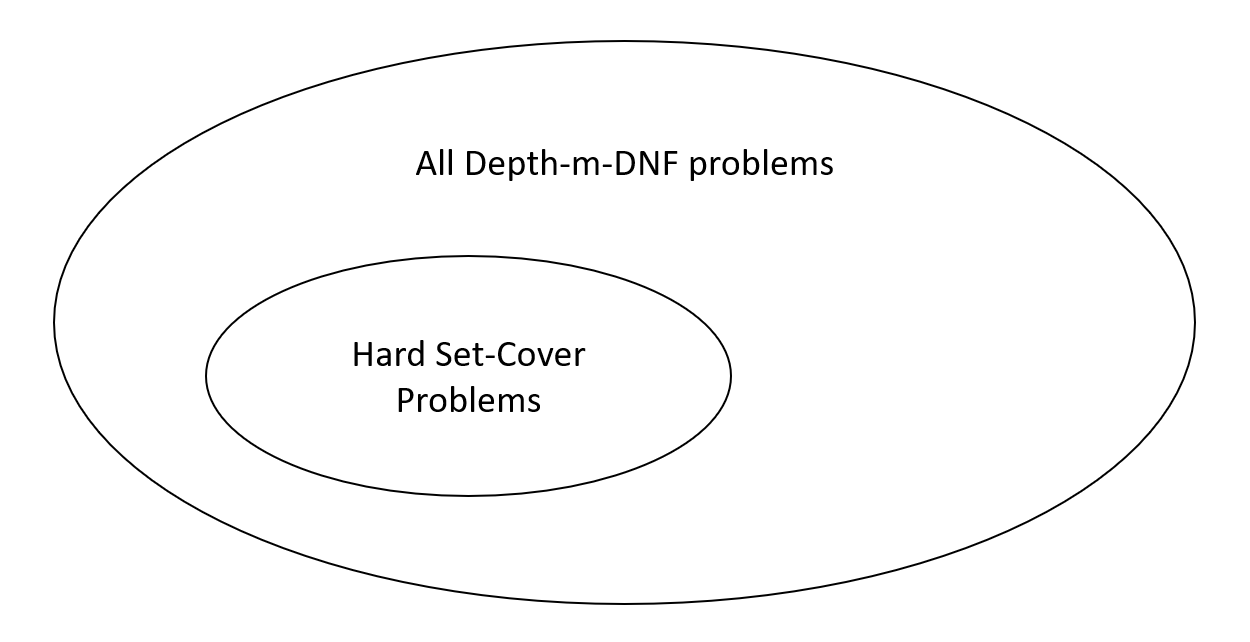
\includegraphics[width=0.5\linewidth]{grafik.png}
    \caption{\textsc{depth-m-dnf} is a more general, possibly harder problem than \textsc{set-cover}}
    \label{fig:enter-label}
\end{figure}

We can show that solving \textsc{set-cover} is basically the same problem as some \textsc{depth-m-dnf} problems. This would show that some instances of \textsc{depth-m-dnf} are just as hard to solve as the hard \textsc{set-cover} problem. A program that solves all \textsc{depth-m-dnf} problems would therefore also have to solve the hard \textsc{set-cover} problems making \textsc{depth-m-dnf} at least as difficult as \textsc{set-cover}. Showing that one problem (\textsc{set-cover}) is a `sub-problem' of another problem (\textsc{depth-m-dnf}) is called a reduction (from \textsc{set-cover} to \textsc{depth-m-dnf}).

\paragraph{The reduction}

Given any \textsc{set-cover} problem we can translate it into a \textsc{depth-m-dnf} problem. We can then also translate it back, thus showing that the problems are basically the same. The \textsc{set-cover} problem can be written in a table, where every cell denotes, whether the set at the top covers the letter on the left, like this:

\begin{center}
    \begin{tabular}{c || c c c | c}
          & $\{a, b\}$ & $\{b\}$ & $\{c, d\}$ & $\{a, b, c, d\}$ \\
          & $\sigma_1$ & $\sigma_2$ & $\sigma_3$ & S' \\
        \hline
        \hline
        a & covered & not covered & not covered & $\rightarrow$ covered \\
        b & covered & covered & not covered & $\rightarrow$ covered \\
        c & not covered & not covered & covered & $\rightarrow$ covered \\
        d & not covered & not covered & covered & $\rightarrow$ covered
    \end{tabular}
\end{center}



We will try to choose some $\sigma$, corresponding to a column, such that each row contains `covered' at least once. Since the rows correspond to each element of S', we have then found a cover for S'. A cover for m=2 is $\sigma_1$ and $\sigma_3$ as established earlier.


\begin{center}
    \begin{tabular}{c || c c c | c}
          & $\{a, b\}$ & $\{b\}$ & $\{c, d\}$ & $\{a, b, c, d\}$ \\
          & \cellcolor{blue!25}$\sigma_1$ & $\sigma_2$ & \cellcolor{blue!25}$\sigma_3$ & S' \\
        \hline
        \hline
        \cellcolor{blue!25}a & \cellcolor{blue!25}covered & not covered & \cellcolor{blue!10}not covered & $\rightarrow$ covered \\
        \cellcolor{blue!25}b & \cellcolor{blue!25}covered & covered & \cellcolor{blue!10}not covered & $\rightarrow$ covered \\
        \cellcolor{blue!25}c & \cellcolor{blue!10}not covered & not covered & \cellcolor{blue!25}covered & $\rightarrow$ covered \\
        \cellcolor{blue!25}d & \cellcolor{blue!10}not covered & not covered & \cellcolor{blue!25}covered & $\rightarrow$ covered
    \end{tabular}
\end{center}

The equivalent \textsc{depth-m-dnf} problem would look like this:

\begin{center}
    \begin{tabular}{c || c c c | c}
        & $\sigma_1$ & $\sigma_2$ & $\sigma_3$ & $y$ \\
        \hline
        \hline
        a & 0 & 1 & 1 & 0 \\
        b & 0 & 0 & 1 & 0 \\
        c & 1 & 1 & 0 & 0 \\
        d & 1 & 1 & 0 & 0
    \end{tabular}
\end{center}


`Covered' has been replaced by 0 and `not covered' by 1.\footnote{That's a bit counter-intuitive, as one might expect it the other way around, but it is caused by the structure of DNFs. The other way around would not work that well. You can try and see what would come out of it.}

As we can see, the solution of choosing $\sigma_1$ and $\sigma_3$ would also be a solution to our DNF problem: $\sigma_1 \land \sigma_3$ would be a (single-and-clause-) DNF, that calculates each y correctly.

However, there is one small problem. This showed that a solution of the \textsc{set-cover} can be translated to the DNF problem, but not the other way around.
In fact, $\sigma_1 \land \lnot\sigma_2$ and even $\bot$ would be valid solution to the DNF problem, but not to the \textsc{set-cover} problem.\footnote{The corresponding solutions to the set cover problem would be to choose $\sigma_1$ and $S'\setminus\sigma_2$ or $S'\setminus\{\}$, which do build proper set covers, but the chosen elements aren't in the set $\Sigma$}

To translate back, we need one more line in our table, that ensures we don't use negations.  The equivalent DNF problem becomes:


\begin{center}
    \begin{tabular}{c || c c c | c}
          & $\sigma_1$ & $\sigma_2$ & $\sigma_3$ & $y$ \\
        \hline
        \hline
        a & 0 & 1 & 1 & 0 \\
        b & 0 & 0 & 1 & 0 \\
        c & 1 & 1 & 0 & 0 \\
        d & 1 & 1 & 0 & 0 \\
        1 & 1 & 1 & 1 & 1
    \end{tabular}
\end{center}

Now solutions, such as $\sigma_1 \land \lnot\sigma_2$, are no longer possible and we will also arrive at a DNF like $\sigma_1 \land \sigma_3$, which can be translated back to \textsc{set-cover}. Since length and depth of any single-and-clause-DNF are the same, we have also shown that \textsc{length-m-dnf} is hard to solve.\footnote{For this last part we assumed that the DNF can always be written as a single-and-clause-DNF, which is not at all obvious and only works, due to our 0 and 1 choices. Feel free to pause and ponder why, if we find a solution to the DNF problem, it can be reduced to a single-and-clause-DNF.}

\end{document}